\section{Apartado A}
\subsection{Diseño del Código de Andamiaje}
\subsection*{Introducción}
El concepto de \enquote{código de andamiaje} en el diseño orientado a objetos, 
particularmente en Java, hace referencia al conjunto de estructuras y métodos 
necesarios para implementar asociaciones entre clases, asegurando la 
consistencia y la integridad del sistema.\par
\vspace{0.15cm}
Su propósito es proporcionar un marco inicial sobre el que los desarrolladores pueden 
construir las funcionalidades particulares de un proyecto. Sin embargo, la línea entre
\enquote{andamiaje} e \enquote{implementación completa} puede ser fina ya que estamos 
añadiendo nuevas funcionalidades que luego se convierten en el nuevo marco inicial para 
futuros cambios que vayamos a realizar en los próximos apartados. A continuación se 
exponen las decisiones diseño que completan el andamiaje inicial.

\subsection{Análisis de opciones de Diseño}
En esta sección se exponen las diferentes opciones de diseño para la implementación 
del sistema de gestión de un refugio de animales, conforme al modelo de clases y 
operaciones proporcionado.\par
\vspace{0.15cm}
El sistema requiere gestionar los socios del refugio (quienes pueden desempeñar 
diferentes roles como voluntarios, donantes y adoptantes), así como el registro, 
adopción y donación de animales. Además, se deben considerar las relaciones entre 
las entidades (socios, animales, refugio, donaciones) y las restricciones del sistema, 
como la consistencia en los datos y las operaciones.\par
\vspace{0.15cm}
Importante mencionar que en nuestro diseño, \textbf{no hemos aplicado un único enfoque de manera 
exclusiva}. Hemos adoptado una combinación de estrategias dependiendo de las necesidades de 
cada relación dentro del sistema justificándolo de forma adecuada.

\subsubsection{Manejo de las Asociaciones}

\begin{description}
    \item[a)] \textbf{Asociación Directa (Sin Reificación\footnote{
        La reificación es una técnica en programación 
        orientada a objetos que se basa en convertir un 
        concepto abstracto, como una relación, en una 
        entidad concreta o clase.})}
\end{description}

\textit{\textbf{Descripción:}}  
En este enfoque, las asociaciones entre clases se implementan directamente como atributos 
en las clases relacionadas.\par
\vspace{0.15cm}
Esta práctica es fácil de implementar porque la cantidad de clases a gestionar 
y el número de clases necesarias para representar las relaciones es menor. No obstante, 
añadir atributos adicionales a las asociaciones (como fechas en el proceso 
de adopción) puede traer problemas de consistencia al manejar relaciones complejas como la 
de un socio con múltiples roles (lo exploraremos en futuras secciones).\par
\newpage % Para que no se ve aglomerada la definición en la footnote
\textbf{Ejemplo: Implementación de \texttt{Refugio} con asociación directa a \texttt{Animal}}\par
La asociación es directa porque \texttt{Refugio} gestiona los \texttt{Animales} mediante varios 
\texttt{Set}, sin una clase intermedia que relacione ambas entidades. (ver Código~\ref{codigo:refugio})\par

En nuestra implementación, hemos decidido la utilización de un \texttt{Set} para las estructuras de datos 
en vez de \texttt{List} en algunos casos por las razones que se detallan en \ref{page:Consideraciones}

Por ejemplo, podríamos añadir la siguiente condición para evitar que un socio pertenezca varias veces a uno o varios refugios:
\begin{lstlisting}[style = javaEspecifico, language=Java]
    if(!s.getRefugio().equals(this)){
    System.out.println("El socio ya esta asociado a otro refugio.");
    return;
}
\end{lstlisting}
El uso de \texttt{Set} nos ahorra esa comprobación añadiendo que hemos asumido que \textbf{solo puede haber un refugio}, entonces esta comprobación deja de ser necesaria. Sin embargo,
en colecciones donde no necesitamos hacer esta clase de comprobación, se usan \texttt{ArrayList}.
\vspace{0.45cm}

\begin{description}
    \item[b)] \textbf{Reificación de la Asociación (Clase de Asociación)}
\end{description}

\textit{\textbf{Descripción:}}  
En este enfoque, las asociaciones complejas entre clases se modelan mediante clases 
intermedias. Por ejemplo, la clase \texttt{Adopcion} representa la relación entre un 
\texttt{Animal}, un \texttt{Adoptante}, y un \texttt{Voluntario}, incluyendo atributos 
como \texttt{fecha} de adopción para capturar detalles específicos de la relación.\par
\vspace{0.15cm}
Como la reificación nos permite agregar atributos y métodos específicos a las relaciones,
facilita la implementación de restricciones complejas relacionadas con la asociación.
Sin embargo, aumenta el número de clases y relaciones a gestionar, lo que hace el diseño más denso
ya que debemos implementar y gestionar las clases de asociación, así como los métodos para 
acceder a las relaciones.\par
\vspace{0.15cm}

\textbf{Nuestra Implementación: Uso de \texttt{Adopcion} como clase de asociación:}
\begin{itemize}
    \item Se representa la relación entre \texttt{Animal}, \texttt{Adoptante} y 
    \texttt{Voluntario} mediante una clase intermedia. (ver Código~\ref{codigo:adopcion})
    \item Atributos como \texttt{fecha} añaden flexibilidad al modelo, permitiendo 
    capturar detalles adicionales de la relación.
    \item Se gestionan las relaciones bidireccionales entre las entidades involucradas, 
    asegurando consistencia en los datos.
\end{itemize}




\subsubsection{Manejo de Roles de los Socios}

\begin{description}
    \item[a)] \textbf{Subclases Específicas para cada Rol}
\end{description}

\textit{\textbf{Descripción:}}  
Cada rol (\texttt{Voluntario}, \texttt{Donante}, \texttt{Adoptante}) se implementa como una 
subclase de la clase \texttt{Socio}. Esto permite encapsular los atributos y métodos 
específicos de cada rol dentro de su respectiva subclase.
\vspace{0.15cm}


Esto proporciona claridad al diseño, ya que cada rol está claramente representado con 
métodos específicos para su comportamiento. Además, permite encapsular los atributos y 
métodos particulares de cada tipo de socio, lo que mejora la organización y legibilidad 
del código. Aunque tiene una limitación significativa para manejar roles múltiples, ya que no permite que 
un socio asuma más de un rol sin duplicar instancias de las subclases. Esto hace que el 
diseño sea rígido y menos flexible en casos donde los roles pueden cambiar dinámicamente 
o coexistir (volveremos a hablar de esto en los siguientes apartados).\par
\vspace{0.15cm}



\textbf{Ejemplo: Subclases específicas para los roles}\par
El diseño tiene implementadas las subclases \texttt{Donante}, \texttt{Adoptante}, 
y \texttt{Voluntario} como extensiones de la clase \texttt{Socio}.\par
(ver Código~\ref{codigo:donante}, \ref{codigo:adoptante}, \ref{codigo:voluntario})

\begin{description}
    \item[b)] \textbf{Uso de Composición de Roles}
\end{description}

\textit{\textbf{Descripción:}}  
En lugar de modelar cada rol como una subclase de \texttt{Socio}, este enfoque utiliza 
la composición para permitir que un socio tenga múltiples roles simultáneamente. 
\vspace{0.15cm}


Este enfoque es mucho más flexible, ya que permite asignar múltiples roles a un socio 
sin necesidad de crear combinaciones de subclases. También simplifica el manejo de 
roles dinámicos y permite cambios en tiempo de ejecución.
Puede reducir la claridad del diseño, ya que no existe una distinción explícita entre 
los diferentes tipos de socios. Además, requiere implementar lógica adicional para 
validar qué operaciones son aplicables para los roles asignados a cada socio.\par
\vspace{0.15cm}


\textbf{Nuestra implementación: Uso de Subclases Específicas para cada Rol:}\par  
\vspace{0.15cm}
Hemos decidido no cambiar como están implementados los roles mediante subclases específicas 
(para este apartado) en lugar de composición. Esto se debe a que en nuestro modelo actual, 
los roles están claramente definidos y no se requiere que un socio tenga múltiples roles de 
manera simultánea. Además:
\begin{itemize}
    \item La claridad y encapsulación que proporciona la herencia permiten manejar las responsabilidades y comportamientos específicos de cada tipo de socio.
    \item Aunque la composición sería más flexible, introducirá complejidad adicional innecesaria para la implementación actual.
\end{itemize}

No obstante, los requisitos del sistema cambiarán en futuros apartados pidiendo que un socio
tenga múltiples roles simultáneamente. En el apartado correspondiente, se discute porque 
la composición sería una solución más adecuada y como se ha implementado.




\subsubsection{Consistencia y Gestión de Datos}\label{page:Consistencia y Gestión de Datos}

\begin{description}
    \item[a)] \textbf{Encapsulación Estricta}
\end{description}

\textit{\textbf{Descripción:}}  
Este enfoque restringe el acceso directo a los atributos y métodos de las clases mediante 
el uso de distintas visibilidades. Para interactuar con los atributos, se proporcionan métodos 
 controlados (\texttt{getters} y \texttt{setters}) que incluyen validaciones (mediante 
\texttt{asserts}) para garantizar que los datos se mantengan en un estado consistente.
Facilita la incorporación de validaciones o pruebas unitarias lo que completa el comportamiento
esperado del sistema. 
\vspace{0.15cm}


\textbf{Ejemplo en el sistema: Uso de encapsulación estricta en la clase \texttt{Refugio}:}\par  
En nuestro sistema, la clase \texttt{Refugio} utiliza atributos privados y distintas visibilidades de métodos 
 garantizar consistencia y control en tiempo de ejecución. ver en Código~\ref{codigo:refugio} como distintos métodos tienen visibilidades especificas para el rol que deben cumplir.
 En \ref{page:Consideraciones} se explican a detalle la función de cada una de las visibilidades presentes.


\begin{description}
    \item[b)] \textbf{Uso de Colecciones Inmutables}
\end{description}

\textit{\textbf{Descripción:}}  
En este enfoque, las colecciones utilizadas para representar relaciones (por ejemplo, 
listas o conjuntos de \texttt{Animal} en \texttt{Refugio}) son inmutables. Esto garantiza 
que las relaciones no puedan ser modificadas accidentalmente fuera de las clases que las 
gestionan.
\vspace{0.15cm}

    Mejora la integridad del sistema al garantizar que las relaciones no se modifiquen de 
    manera no controlada.
    Por otro lado introduce rigidez ya que no permite realizar cambios dinámicos en las relaciones sin 
    reemplazar completamente la colección. Esto puede dificultar la gestión de operaciones 
    como agregar o eliminar elementos.\par
    \vspace{0.15cm}

\textbf{Ejemplo de Uso de Colecciones Inmutables en la Clase \texttt{Refugio}:}\par  
En nuestro sistema, el método \texttt{getAnimalesRegistrados} de la clase \texttt{Refugio} 
devuelve una vista inmutable de los animales registrados. Esto asegura que los \texttt{Set} no 
puedan modificarse ya que el uso de \texttt{Collections.}\texttt{enumeration} 
garantiza que la colección de animales no pueda ser alterada fuera de la clase \texttt{Refugio}, 
manteniendo la consistencia de los datos. (ver Código~\ref{codigo:refugio} como ejemplo aunque se implementa esta práctica en varias clases del sistema)

\textbf{Decisión Tomada: Encapsulación Controlada con Enumerations:}\par
En nuestro diseño, optamos por una encapsulación controlada en lugar de colecciones 
completamente inmutables. Utilizar enumeraciones en los métodos \texttt{get} garantiza que las colecciones 
no se modifiquen desde fuera de las clases, preservando la integridad de los datos.

Este enfoque combina lo mejor de ambos mundos: flexibilidad para realizar cambios controlados 
y protección contra modificaciones accidentales en las estructuras de datos.

\subsubsection{Representación de Relaciones en el Sistema}

\begin{description}
    \item[a)] \textbf{Relaciones Unidireccionales}
\end{description}

\textit{\textbf{Descripción:}}  
En una relación unidireccional, solo una entidad tiene conocimiento de la relación. 
Por ejemplo, un \texttt{Adoptante} puede conocer al \texttt{Animal} que adopta, 
pero el \texttt{Animal} no necesita saber nada sobre el \texttt{Adoptante}.\par
\vspace{0.15cm} 
Estas relaciones gestionan la relación con una clase, lo que reduce la complejidad del sistema.
El problema, es que limita las consultas entre clases relacionadas y puede volverse más complejo 
añadir funcionalidades.\par
\vspace{0.15cm}

\begin{description}
    \item[b)] \textbf{Relaciones Bidireccionales}
\end{description}

\textit{\textbf{Descripción:}}  
En una relación bidireccional, ambas entidades conocen y mantienen referencias mutuas. 
Por ejemplo, cuando un \texttt{Adoptante} adopta un \texttt{Animal}, ambos se actualizan 
mutuamente para reflejar la relación.\par
\vspace{0.15cm}
Las relaciones de este estilo garantizan la consistencia de los datos, ya que ambas partes relacionadas están 
sincronizadas al mantener referencias mutuas explícitas. Sin embargo, como hay que tener una sincronización constante 
entre las todas las clases relacionadas, si tuviéramos muchas relaciones bidireccionales puede dificultar el mantenimiento
por que genera un alto nivel de acoplamiento.\par
\vspace{0.15cm}
\textbf{Ejemplo en el Sistema: Relaciones Bidireccionales en \texttt{Adopcion}}\par 
En nuestro diseño, la relación entre \texttt{Animal}, \texttt{Adoptante}, y 
\texttt{Voluntario} es bidireccional y se asegurando consistencia en ambas direcciones
reflejando los cambios realizados en una clase en las demás involucradas.
(ver Código~\ref{codigo:adopcion} como, por ejemplo, se actualiza el estado del animal tras ser adoptado)\par
\vspace{0.15cm}
\textbf{Decisión Tomada:}\par
Hemos implementado relaciones bidireccionales para las asociaciones complejas del sistema, 
como las adopciones, ya que garantizan consistencia y sincronización entre las entidades 
relacionadas. Sin embargo, para relaciones más simples, como la lista de animales en un 
refugio, usamos relaciones unidireccionales para mantener la simplicidad.


\newpage
\subsection{Diagrama de Diseño}

\begin{figure}[H]
    \centering
     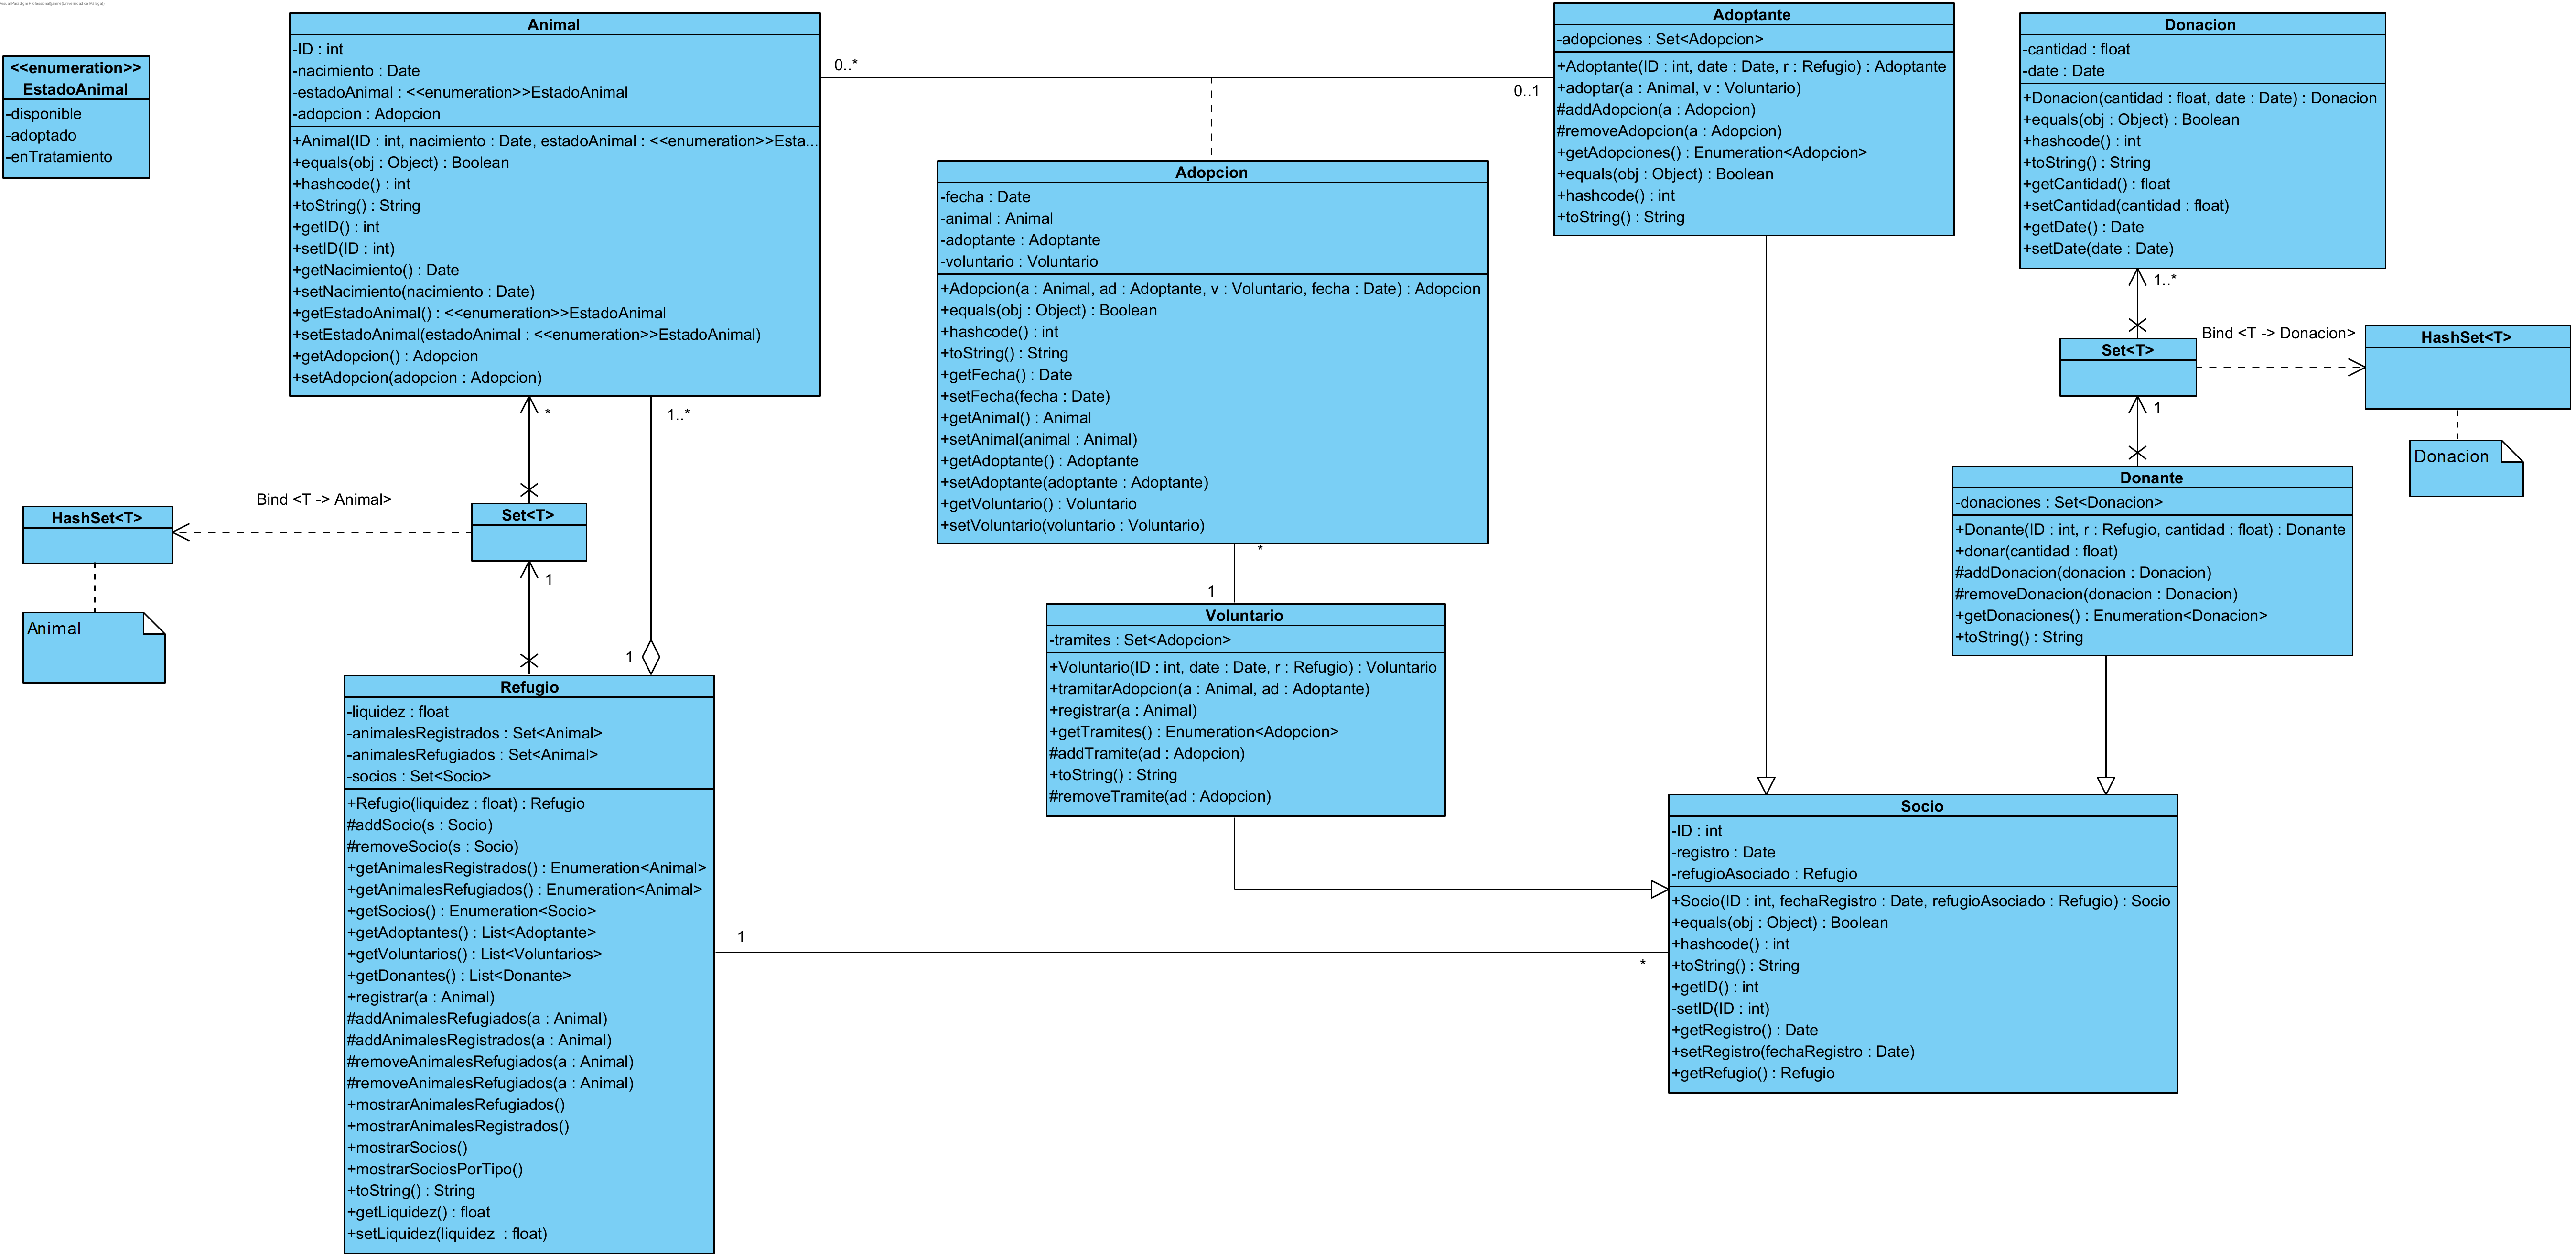
\includegraphics[width=1\linewidth]{assets/Diagrama_bien.png}
     \caption{Diagrama de Diseño del apartado A}
\end{figure}

Este es un diagrama enriquecido en el que se muestran las relaciones, productos, operaciones y funciones de todas las clases.

\subsection{Consideraciones}\label{page:Consideraciones}

Aquí tienes el párrafo reestructurado y enumerado correctamente, manteniendo los itemize correspondientes:

\begin{description}
    \item[1.] \textbf{Gestión de relaciones:}
\end{description}
Las relaciones (1..*) que tenemos se han gestionado usando un \texttt{Set} en cada una por las siguientes razones:
\begin{itemize}
    \item \textbf{Control de elementos repetidos:} Los \texttt{Set} usan los métodos de \texttt{hashCode} e \texttt{equals}
    para hacer la comprobación de la existencia de elementos en la colección. Si un nuevo elemento coincide con uno existente, 
    no se inserta, evitando comprobaciones adicionales que haríamos con el uso de \texttt{List} mediante \texttt{asserts}. En 
    nuestro caso, \texttt{equals} hace comprobación de la existencia de un animal mediante el tipo e ID de la instancia.
    \item \textbf{Complejidad algorítmica:} En los \texttt{HashSet}, la búsqueda y la inserción tienen una complejidad de \(O(1)\), 
    ya que se basan en tablas hash. Por otro lado, en una \texttt{List} (como \texttt{ArrayList}), las operaciones de búsqueda tienen una 
    complejidad de \(O(n)\), porque requiere iterar sobre los elementos que es la misma en el peor de los casos para el \texttt{HashSet} si hay muchas colisiones en la tabla hash.
    \item \textbf{Orden de los elementos:} En nuestra implementación, no es necesario mantener un orden específico en las colecciones. 
    Por esta razón, el uso \texttt{Set} es más adecuado que \texttt{List} teniendo en cuenta los puntos anteriores.
\end{itemize}

\begin{description}
    \item[2.] \textbf{Encapsulación y visibilidad de métodos:}
\end{description}
En distintas clases del sistema, se puede apreciar el uso de métodos públicos, privados y protegidos siguiendo los lineamientos de la Encapsulación Directa \ref{page:Consistencia y Gestión de Datos}.
Las funcionalidad que cada visibilidad implementa en el código:
\begin{itemize}
    \item \textbf{public} permite el acceso desde cualquier clase del programa.
    \item \textbf{private} solo hace accesible el método dentro de la misma clase.
    \item \textbf{protected} hace el método accesible a clases dentro del mismo paquete.
\end{itemize}
En nuestra implementación decidimos utilizar visibilidades \texttt{protected} con métodos que modifican las colecciones de datos mediante \texttt{add} o \texttt{remove} 
para evitar modificaciones indeseadas.\par
\vspace{0.20cm}

\begin{description}
    \item[3.] \textbf{Representación de atributos de precio:}
\end{description}
En distintas clases hacemos referencia a \textbf{liquidez} como un \texttt{float} porque al estar tratando con dinero, vamos a tener como máximo de dos decimales. Usar un \texttt{double} es malgastar  memoria que no es necesaria.
\vspace{0.20cm}

\begin{description}
    \item[4.] \textbf{Control de restricciones:}
\end{description}
Controlamos las restricciones mediante el uso de \texttt{assert} los cuales permiten validar que ciertas condiciones se cumplan durante la ejecución del programa. Si una restricción no se cumple, se lanza un error en tiempo de ejecución, lo que ayuda a detectar inconsistencias.


\newpage



\subsection{Implementación del Modelo}
\subsubsection{Clase Socio}
La clase \texttt{Socio} es abstracta y representa la base para las distintas subclases: 
\texttt{Adoptante}, \texttt{Voluntario}, y \texttt{Donante}. Esta clase asegura que 
cada socio tenga un \texttt{ID} único, una fecha de registro válida y un refugio asociado.
\label{codigo:socio}
\begin{lstlisting}[style = javaNormal, language=Java] 
public abstract class Socio {
    private int ID; 
    private Date fecha;
    private final Refugio refugioAsociado;

    public Socio(int ID, Date fecha, Refugio refugioAsociado) {
        assert ID > 0 : "El ID del socio debe ser valido.";
        assert fecha != null : "La fecha de registro no puede ser nula.";
        assert refugioAsociado != null : "El refugio asociado no puede ser nulo.";
        this.ID = ID;
        this.fecha = fecha;
        this.refugioAsociado = refugioAsociado;
    }
    public int getID() {
        return ID;
    }
    public Date getDate() {
        return this.fecha;
    }
    public Refugio getRefugio() {
        return this.refugioAsociado;
    }
}
\end{lstlisting}
\label{codigo:donante}
\subsubsection{Clase Donante}
La clase \texttt{Donante} extiende de \texttt{Socio} y gestiona las donaciones realizadas 
por un socio. Las donaciones se almacenan en un \texttt{Set} para evitar duplicados.

\begin{lstlisting}[style = javaNormal, language=Java] 
public class Donante extends Socio {
    private Set<Donacion> donaciones;

    public Donante(int ID, Date date, Refugio r, Double cantidad) {
        super(ID, date, r);
        assert cantidad > 0 : "La cantidad inicial donada debe ser mayor a cero.";
        donaciones = new HashSet<>();
        this.donar(cantidad);
    }

    public void donar(Double cantidad) {
        assert cantidad > 0 : "La cantidad donada debe ser mayor a cero.";
        LocalDate fechaDonacion = LocalDate.now();
        Donacion d = new Donacion(cantidad, Date.from(fechaDonacion.atStartOfDay(ZoneId.systemDefault()).toInstant()), this);
        donaciones.add(d);
        Refugio r = super.getRefugio();
        r.setLiquidez(r.getLiquidez() + cantidad);
        r.addSocio(this);
        assert donaciones.contains(d);
    }
}
\end{lstlisting}

\subsubsection{Clase Adoptante}
La clase \texttt{Adoptante} extiende de \texttt{Socio} y gestiona las adopciones realizadas 
por un adoptante. Las adopciones se almacenan en un \texttt{Set}.
\label{codigo:adoptante}
\begin{lstlisting}[style = javaNormal, language=Java] 
public class Adoptante extends Socio {
    private Set<Adopcion> adopciones;

    public Adoptante(int ID, Date date, Refugio r) {
        super(ID, date, r);
        adopciones = new HashSet<>();
    }

    public void adoptar(Animal a, Voluntario v) {
        assert !adopciones.stream().anyMatch(ad -> ad.getAnimal().equals(a)) : "El adoptante ya tiene registrado este animal";
        v.tramitarAdopcion(a, this);
    }

    public void addAdopcion(Adopcion a) {
        adopciones.add(a);
    }
}
\end{lstlisting}

\subsubsection{Clase Voluntario}
La clase \texttt{Voluntario} extiende de \texttt{Socio} y gestiona los trámites de 
adopción realizados por un voluntario.
\label{codigo:voluntario}
\begin{lstlisting}[style = javaNormal, language=Java] 
public class Voluntario extends Socio {
    Set<Adopcion> tramites;

    public Voluntario(int ID, Date date, Refugio r) {
        super(ID, date, r);
        tramites = new HashSet<>();
    }

    public void tramitarAdopcion(Animal a, Adoptante ad) {
        assert a.getEstadoAnimal() == EstadoAnimal.DISPONIBLE : "El animal ya esta adoptado.";
        LocalDate fechaAdopcion = LocalDate.now();
        Adopcion adopcion = new Adopcion(a, ad, this, Date.from(fechaAdopcion.atStartOfDay(ZoneId.systemDefault()).toInstant()));
        tramites.add(adopcion);
    }
}
\end{lstlisting}

\subsubsection{Clase Refugio}
La clase \texttt{Refugio} gestiona el conjunto de \texttt{Socios} y \texttt{Animales}. 
Las operaciones están centralizadas para simplificar la gestión.
\label{codigo:refugio}
\begin{lstlisting}[style = javaNormal, language=Java] 
public class Refugio {
    private double liquidez;
    private Set<Animal> animalesRegistrados;
    private Set<Socio> socios;

    public Refugio(double liquidez) {
        assert liquidez >= 0 : "La liquidez debe ser no negativa.";
        this.liquidez = liquidez;
        animalesRegistrados = new HashSet<>();
        socios = new HashSet<>();
    }

    public void addSocio(Socio s) {
        assert s != null : "El socio no puede ser nulo.";
        socios.add(s);
    }
}
\end{lstlisting}

\subsubsection{Clase Donacion}
La clase \texttt{Donacion} representa una donación realizada por un \texttt{Donante}. 
Incluye la cantidad, la fecha de la donación y el donante asociado. Las validaciones 
aseguran que los valores sean válidos en el momento de la creación de la instancia.
\label{codigo:donacion}
\begin{lstlisting}[style = javaNormal, language=Java] 
public class Donacion {
    private Double cantidad;
    private Date date;
    private final Donante donante;

    public Donacion(Double cantidad, Date date, Donante donante) {
        assert cantidad != null && cantidad > 0 : "La cantidad debe ser positiva.";
        assert date != null && !date.after(new Date()) : "La fecha no puede ser nula ni estar en el futuro.";
        assert donante != null : "El donante no puede ser nulo.";
        this.cantidad = cantidad;
        this.date = date;
        this.donante = donante;
    }

    public Double getCantidad() {
        assert cantidad != null && cantidad > 0 : "La cantidad no puede ser nula.";
        return cantidad;
    }

    public void setCantidad(Double cantidad) {
        this.cantidad = cantidad;
    }

    public Date getDate() {
        assert date != null : "La fecha no puede ser nula.";
        return date;
    }

    public void setDate(Date date) {
        this.date = date;
    }

    public Donante getDonante() {
        return this.donante;
    }

    @Override
    public String toString() {
        return String.format("Donacion: %.2f, %tY-%tB-%td", cantidad, date, date, date);
    }
}
\end{lstlisting}
\label{codigo:adopcion}
\subsubsection{Clase Adopcion}
La clase \texttt{Adopcion} modela una adopción de un \texttt{Animal} realizada por un 
\texttt{Adoptante}, gestionada por un \texttt{Voluntario}. Implementa la bidireccionalidad 
entre estas entidades para mantener consistencia en las asociaciones.

\begin{lstlisting}[style = javaNormal, language=Java] 
public class Adopcion {
    private Date fecha;
    final private Animal animal;
    final private Adoptante adoptante;
    final private Voluntario voluntario;

    public Adopcion(Animal a, Adoptante ad, Voluntario v, Date fecha) {
        assert a != null : "El animal no puede ser nulo.";
        assert ad != null : "El adoptante no puede ser nulo.";
        assert v != null : "El voluntario no puede ser nulo.";
        assert a.getEstadoAnimal() == EstadoAnimal.DISPONIBLE : "El animal debe estar disponible para adopcion.";
        assert fecha != null && !fecha.after(new Date()) : "La fecha no puede ser nula ni estar en el futuro.";

        this.animal = a;
        this.adoptante = ad;
        this.voluntario = v;
        this.fecha = fecha;

        a.setEstadoAnimal(EstadoAnimal.ADOPTADO);
        ad.addAdopcion(this);
        assert Collections.list(ad.getAdopciones()).contains(this) : 
        "La adopcion no fue anadida correctamente al adoptante.";
        v.addTramite(this);
        assert Collections.list(v.getTramites()).contains(this) : 
        "La adopcion no fue anadida correctamente al voluntario.";
    }

    public Date getFecha() {
        return this.fecha;
    }

    public void setFecha(Date fecha) {
        assert fecha != null && !fecha.after(new Date()) : "La fecha no puede ser nula ni estar en el futuro";
        this.fecha = fecha;
    }

    public Animal getAnimal() {
        return this.animal;
    }

    public Voluntario getVoluntario() {
        return this.voluntario;
    }

    public Adoptante getAdoptante() {
        return this.adoptante;
    }

    @Override
    public String toString() {
        return String.format("Adopcion: %tY-%tB-%td, %s, %s", fecha, fecha, fecha, animal, adoptante);
    }
}
\end{lstlisting}
\label{codigo:animal}
\subsubsection{Clase Animal}
La clase \texttt{Animal} modela a un animal registrado en el sistema. Cada animal tiene un 
ID único, una fecha de nacimiento, un estado actual y está asociado a un \texttt{Refugio}.

\begin{lstlisting}[style = javaNormal, language=Java] 
public class Animal {
    private int ID;
    private Date nacimiento;
    private EstadoAnimal estadoAnimal;
    final private Refugio refugio;
    private Adopcion adopcion;

    public Animal(int ID, Date nacimiento, EstadoAnimal estadoAnimal, Refugio refugio, Adopcion adopcion) {
        assert ID > 0 : "El ID del animal debe ser valido.";
        assert nacimiento != null : "La fecha de nacimiento no puede ser nula.";
        assert estadoAnimal != null : "El estado del animal debe estar definido.";
        assert refugio != null : "El refugio debe existir.";

        this.ID = ID;
        this.nacimiento = nacimiento;
        this.estadoAnimal = estadoAnimal;
        this.refugio = refugio;
        this.adopcion = adopcion;
    }

    public EstadoAnimal getEstadoAnimal() {
        return estadoAnimal;
    }

    public void setEstadoAnimal(EstadoAnimal estadoAnimal) {
        assert estadoAnimal != null : "El estado del animal debe estar definido.";
        this.estadoAnimal = estadoAnimal;
    }

    public Date getNacimiento() {
        return nacimiento;
    }

    public void setNacimiento(Date nacimiento) {
        assert nacimiento != null : "La fecha de nacimiento no puede ser nula";
        this.nacimiento = nacimiento;
    }

    public Refugio getRefugio() {
        return refugio;
    }

    public Adopcion getAdopcion() {
        return this.adopcion;
    }

    public void setAdopcion(Adopcion adopcion) {
        assert adopcion != null;
        this.adopcion = adopcion;
    }

    @Override
    public String toString() {
        return String.format("Animal: ID=%d, nacimiento=%tF, estado=%s", ID, nacimiento, estadoAnimal);
    }
}
\end{lstlisting}



\subsection{Testing}
Con la siguiente clase hemos comprobado el funcionamiento del sistema:
\begin{lstlisting}[style = javaNormal, language=Java] 

\end{lstlisting}

\subsection{Conclusión}

El diseño e implementación del código de andamiaje para el sistema se realizó siguiendo 
los principios fundamentales del diseño orientado a objetos, adaptados a los requerimientos 
específicos de este apartado. Se tomaron la decisiones de diseño adecuadas, como la gestión 
de asociaciones entre clases, la encapsulación de datos y la validación de restricciones con \texttt{assert}, 
proporcionando un modelo consistente y completo.\par
\vspace{0.15cm}
Una de las decisiones clave fue el uso combinado de asociaciones directas para relaciones 
simples y la reificación de asociaciones para relaciones más complejas junto con métodos \texttt{get}
que devuelven conjuntos inmutables. Esto permitió mantener un equilibrio entre la simplicidad de las 
implementaciones directas, como la gestión de animales en el refugio, y la flexibilidad 
de las relaciones complejas, como las adopciones, donde se requieren atributos adicionales 
y validaciones específicas mientras protegíamos las listas de cada objeto en el sistema.\par
\vspace{0.15cm}
Además, la bidireccionalidad en relaciones como las adopciones, garantizó la 
consistencia del modelo al sincronizar automáticamente los datos entre las
clases participantes.\par

\newpage
